\section{Visualisation tools in ML4PG}\label{sec:visualisation}



\begin{figure}
 
$$
\xy0;/r.12pc/: 
*[o]=<80pt,30pt>\hbox{\txt{Coq libraries:\\one or many?}}="a"*\frm<8pt>{-,},
(40,35)*[o]=<80pt,30pt>\hbox{\txt{General\\pattern-search}}="r"*\frm<8pt>{-},
(40,-35)*[o]=<80pt,30pt>\hbox{\txt{Relative to\\ Coq object}}="b"*\frm<8pt>{-},
(80,55)*[o]=<80pt,15pt>\hbox{\txt{Terms}}="c"*\frm<8pt>{-},
(80,15)*[o]=<80pt,15pt>\hbox{\txt{Proofs}}="d"*\frm<8pt>{-},
(80,-15)*[o]=<80pt,15pt>\hbox{\txt{Terms}}="e"*\frm<8pt>{-},
(80,-55)*[o]=<80pt,15pt>\hbox{\txt{Proofs}}="f"*\frm<8pt>{-},
(160,55)*[o]=<120pt,15pt>\hbox{\txt{Visualise term clusters?}}="g"*\frm<8pt>{-,},
(160,15)*[o]=<120pt,15pt>\hbox{\txt{Visualise proof families?}}="h"*\frm<8pt>{-,},
(160,-15)*[o]=<120pt,15pt>\hbox{\txt{Visualise the term tree?}}="i"*\frm<8pt>{-,},
(160,-55)*[o]=<120pt,15pt>\hbox{\txt{Visualise the proof flow?}}="j"*\frm<8pt>{-,},
"a";"b" **\dir{-} ?>*\dir{>},
"a";"r" **\dir{-} ?>*\dir{>},
"r";"c" **\dir{-} ?>*\dir{>},
"r";"d" **\dir{-} ?>*\dir{>},
"b";"e" **\dir{-} ?>*\dir{>},
"b";"f" **\dir{-} ?>*\dir{>},
"c";"g" **\dir{-} ?>*\dir{>},
"d";"h" **\dir{-} ?>*\dir{>},
"e";"i" **\dir{-} ?>*\dir{>},
"f";"j" **\dir{-} ?>*\dir{>},
%"r";"a" **\dir{-} ?>*\dir{>},
%"c";"d" **\dir{-} ?>*\dir{>},
%"d";"h" **\dir{-} ?>*\dir{>},
%"c";"e" **\dir{-} ?>*\dir{>},
%"e";"c" **\dir{-} ?>*\dir{>}
%+<0em,0em>@+ 
\endxy
$$
\caption{Visualisation techniques included in ML4PG.}\label{fig:visualisation}
\end{figure}


In the previous sections, we have seen how ML4PG can be used to find families of proofs following 
a common pattern, and use those families to automatically prove theorems. However, when the proof-generation
method fails, the output provided by ML4PG algorithms is just a set of similar patches with no hints of why 
these proof-patches are deemed similar. 
% In addition, the user needs
% to replay the proof to infer the pattern. %Therefore, the conceptualisation of proof-patterns can be
% %a challenge. 
In this section, we present our approach to facilitate the understanding of proof patterns using different visualisation tools
that are summarised in Figure~\ref{fig:visualisation}.

\paragraph{An automaton-like representation of the proof-flow}
The first problem that we address is the discovery of the key features that were taken
into account during the cluster formation. This is a well-known problem in machine-learning 
known as \emph{feature selection}~\cite{Bishop}. From a given set of features, feature selection algorithms 
generate different subsets of features and create a ranking of feature subsets.
ML4PG uses the \emph{correlation-based feature subset selection} algorithm implemented in Weka~\cite{Weka}
--- the machine-learning toolbox employed by ML4PG to extract the relevant features.

\begin{example}\label{ex:correlation-features}
In the case study presented at the end of Section~\ref{sec:recurrent}, the relevant features were:

$-$ The tactics applied in the first and second steps of the proof-patches (\lstinline?case? and \lstinline?rewrite? respectively).

$-$ The type of the argument of the tactic applied in the first step of the proof-patches (\lstinline?nat?).

$-$ The second top symbol of the goal in the second step of the proof-patches (the $\sum$ symbol). 

$-$ The first and second auxiliary lemmas applied in the the third step of the proof-patches. The first auxiliary lemma (\lstinline?sumrB?) is used to expand the summations and is 
common to all the proofs. There are two different \lq\lq{}second\rq\rq{} auxiliary lemmas that occur in the proofs of Lemma~\ref{lem:fundamental} and~\ref{lem:nilpotent2} (\lstinline?big_nat_recr? and
\lstinline?big_nat_recl? --- both extract elements of a summation); however, the recurrent feature extraction process have assigned similar values to them.

ML4PG uses this information and produces an automaton-shape representation for discovered % to help in the visualisation of 
proof-patterns and the correlated features that determined the patterns. In our example, the associated ``automaton'' is depicted in Figure~\ref{fig:automata}. 
\end{example}



% This feature selection mechanism helps to explain why the proof-patches are similar since it indicates the 
% features that have been relevant for the construction of the cluster. To show the selected features and their relation with 
% the proof-patches, we introduce an automaton-shape representation. In~\cite{GWR14}, a tool to infer models 
% from proof traces was presented. Those models help to understand the behaviour exhibited by a collection
% of proofs and is represented by automata. 


Generally, given a cluster of proof patches ${\cal C}$, we have an automaton $A$ with $5$ consecutive states. The $i$th state of $A$ is labelled
with the list of $i$th goals in the proof-patches contained in ${\cal C}$. The transitions between the $i$th and $i+1$th states are given by 
the $i$th tactic of each proof-patch of ${\cal C}$. If two or more tactics belong to the same group (see Table~\ref{tab:tactics}),
they are merged in a unique transition; otherwise, the tactics will be shown as different transitions. In addition, each state is annotated with 
features 
whose correlation determined the cluster.

\begin{figure}[t]
\centering 
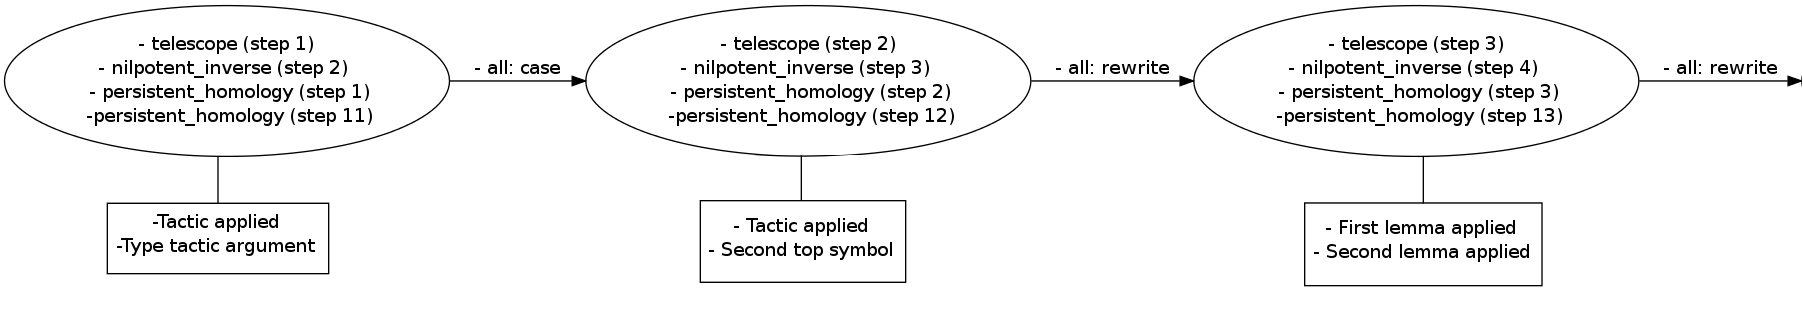
\includegraphics[scale=.19]{itp6.png}
\caption{\scriptsize{\emph{Fragment of the automaton 
 corresponding to the cluster of four lemma fragments described in the case study of Section~\ref{sec:recurrent}} (the whole automaton can be seen in Appendix~\ref{sec:automaton}). 
It shows correspondence between certain proof steps of lemmas % the following lemmas were discovered:
\texttt{telescope} (for the lemma of Example~\ref{example0}), \texttt{nilpotent\_inverse} (for Lemma~\ref{lem:nilpotent2}), and \texttt{persistent\_homology} 
(for Lemma~\ref{lem:fundamental}). Square boxes denote feature correlation where it exists. 
To be compact, we  hide full lemma statements, tactic and auxiliary lemma names, symbols, etc., but they can be shown by ML4PG. 
%For example, the full statements of the following cluster lemmas will be shown:
%The names of the lemmas of that cluster are: 
}}\label{fig:automata}
\end{figure}




\paragraph{A tree representation for terms}

As we have previously explained, ML4PG can cluster terms using a recurrent clustering process (see Section~\ref{sec:reclemmaclustering}). When using this tool, the output generated by ML4PG is a list of names of similar terms, and the user should inspect the libraries to compare the different terms. In order to simplify this process, we have created a visualisation tool that generates the ML4PG term-tree (cf. Definition~\ref{def:ml4pgtermtree}) given the name associated with a term.

\begin{example}
 In Example~\ref{ex:maxnACA}, we have shown how the lemma \lstinline?maxnACA? is automatically proven thanks to its similarity with lemmas \lstinline?addnACA?, \lstinline?minnACA?, \lstinline?mulnACA?. From Figure~\ref{fig:treevisualisation}, it is trivial why these 4 lemmas are similar.

 
 

\begin{figure}
\centering
\begin{tikzpicture}
\draw (0,0) node{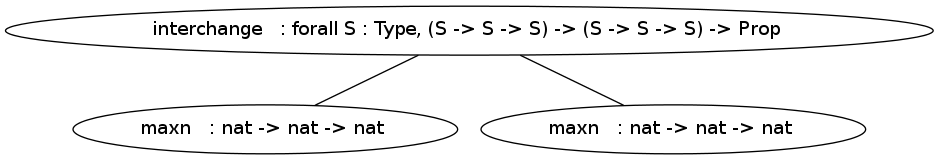
\includegraphics[scale=.2]{maxnACA.png}} ;
\draw (7,0) node{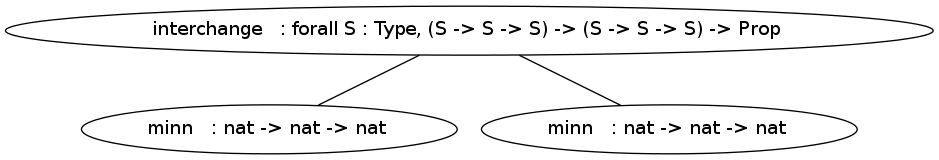
\includegraphics[scale=.2]{minnACA.png}};
\draw (0,-1.5) node{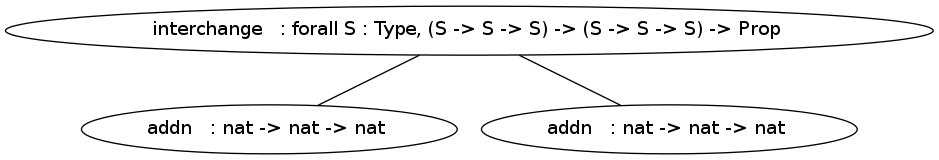
\includegraphics[scale=.2]{addnACA.png}} ;
\draw (7,-1.5) node{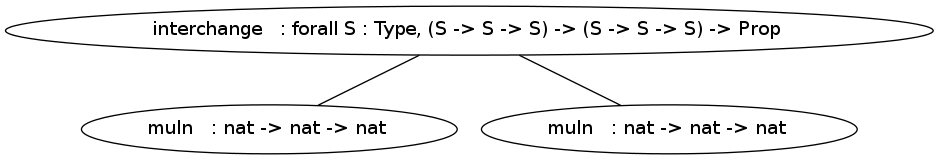
\includegraphics[scale=.2]{mulnACA.png}}  ;
\end{tikzpicture}
\caption{Term trees associated with \texttt{maxnACA} (top left), \texttt{minnACA} (top right), \texttt{addnACA} (bottom left), \texttt{mulnACA} (bottom right).}\label{fig:treevisualisation} 
\end{figure} 
 
 \end{example}

 
\paragraph{Cluster visualisation}

Finally, we have also improved the visualisation of clusters. Initially, ML4PG's output is a list of similar lemmas (or in general terms), and the user can adjust the accuracy of those families varying the granularity value (see the case studied included at the end of Section~\ref{sec:recurrent}). However, this means that he has to run the clustering process several times, and remember the families that were generated in each iteration. These problems have been tackled thanks to a new visualisation tool that captures the relations between the families of similar proofs/terms obtained using different granularity values, see Figure~\ref{fig:clustervisualisation}.




\begin{figure}
\centering
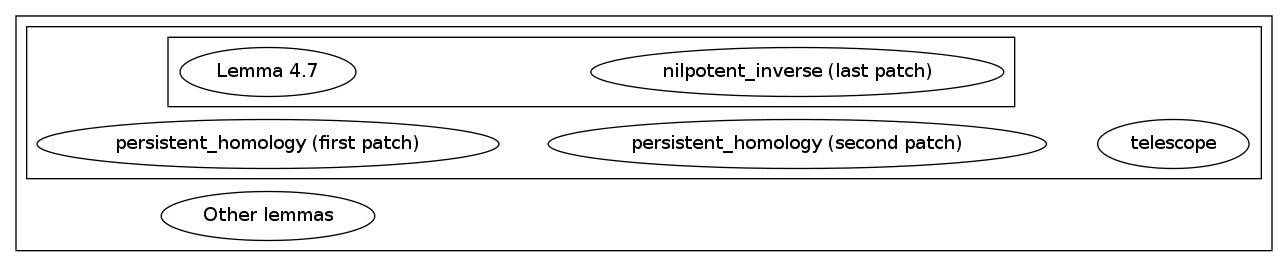
\includegraphics[scale=.3]{clustervisualisation.png}
\caption{Cluster visualisation for the case study included at the end of Section~\ref{sec:recurrent} regarding the families of similar lemmas to Lemma~\ref{lem:nilpotent}: \texttt{telescope} (for the lemma of Example~\ref{example0}), \texttt{nilpotent\_inverse} (for Lemma~\ref{lem:nilpotent2}), and \texttt{persistent\_homology} 
(for Lemma~\ref{lem:fundamental}). The outer, middle and inner square contain, respectively, the proof-patches obtained with granularities 1, 3 and 5. It shows correspondence between certain proof steps of lemmas % the following lemmas were discovered:
}\label{fig:clustervisualisation} 
\end{figure} 



%for clustering that are related to that 
%state.


% $-$ there are several transitions from the $j$th to the $j+1$th state labelled by the $j$th tactic of each proof-patch of $P$ -- if either the $j$th tactic of two or more
% proof-patches is the same or belong to the same group (see Table~\ref{tab:tactics}), the transitions are merged in a unique transition labelled with the set of those tactics,
% 
% $-$ if a proof ends after the $j$th tactic of a proof-patch, the $j+1$ state is represented as final.

%\begin{example}

 
 




%\end{example}


